\subsection{Implémentation du Peer}

Le peer est un élément central du système P2P. Il agit à la fois comme client et serveur.

\subsubsection{Serveur Peer}

Le serveur peer permet d’accepter des connexions entrantes d’autres pairs.

Il est implémenté avec une \textbf{ServerSocket} en Java. 
Chaque nouvelle connexion est gérée dans un thread séparé.

\textbf{Principe :}
\begin{itemize}
    \item Le serveur écoute sur un port donné
    \item Lorsqu’un pair se connecte, un \texttt{PeerHandler} est créé
    \item Chaque handler traite les requêtes indépendamment
\end{itemize}

\begin{figure}[h]
    \centering
    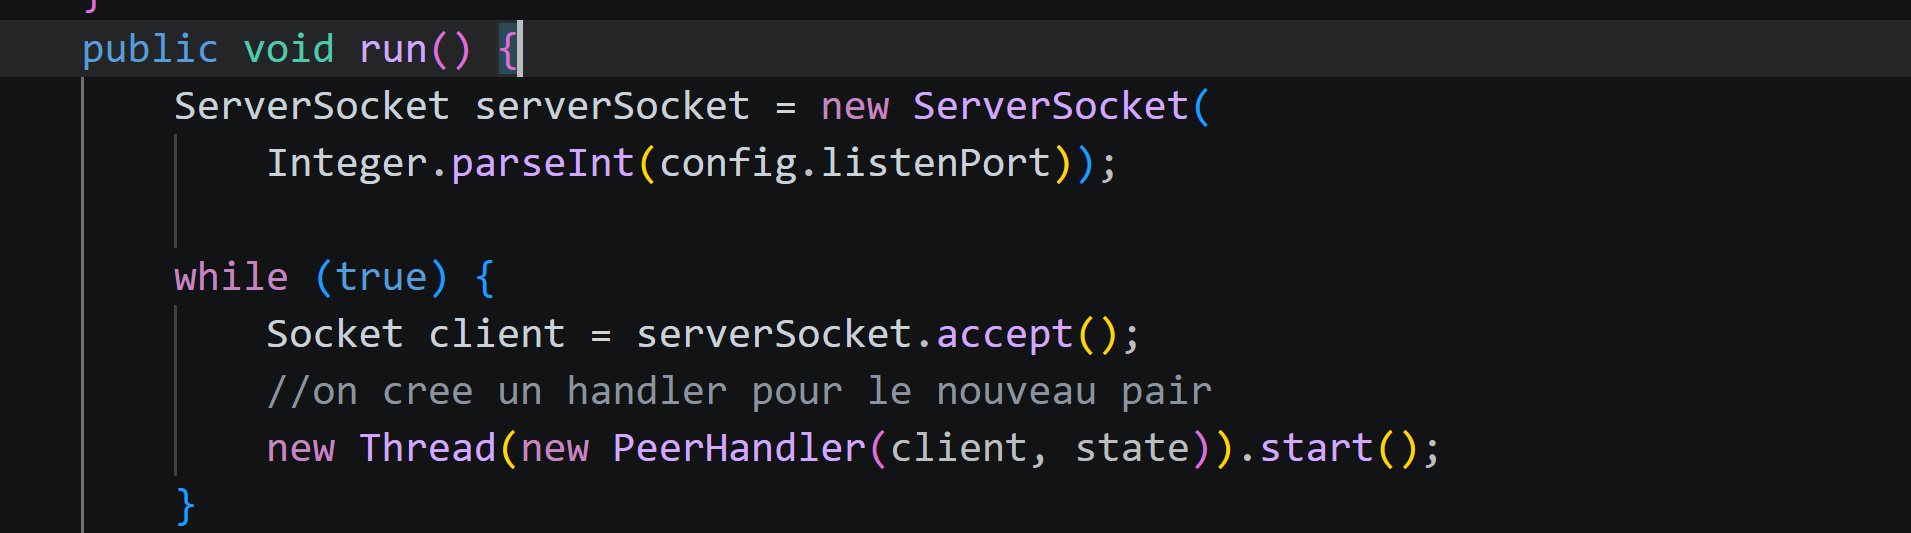
\includegraphics[width=0.7\linewidth]{peerserver.png}
    \caption{Architecture du PeerServer}
    \label{fig:peerserver}
\end{figure}

Cela permet de gérer plusieurs connexions simultanément.

\subsubsection{Gestion des commandes Peer-Peer}

Le \texttt{PeerHandler} gère plusieurs types de messages :

\paragraph{1. interested}
Lorsqu’un pair est intéressé par un fichier, il envoie :

\begin{verbatim}
interested <key>
\end{verbatim}

Le serveur répond avec un \textbf{buffermap} encodé en Base64.

\paragraph{2. have}
Cette commande permet d’échanger les buffermaps entre pairs.

Cela permet de savoir quelles pièces sont disponibles chez chaque voisin.

\paragraph{3. getpieces}
Le peer demande certaines pièces d’un fichier :

\begin{verbatim}
getpieces <key> [index1 index2 ...]
\end{verbatim}

Le serveur :
\begin{itemize}
    \item vérifie qu’il possède les pièces
    \item lit les données dans le fichier
    \item envoie un header + payload binaire
\end{itemize}

\subsubsection{Gestion du buffermap}

Le buffermap est représenté par un \textbf{BitSet} en Java.

\begin{itemize}
    \item 1 = pièce disponible
    \item 0 = pièce absente
\end{itemize}

Il est ensuite encodé en Base64 pour être transmis.

\subsubsection{Client Peer}

Le client permet de communiquer avec le tracker :

\begin{itemize}
    \item connexion TCP
    \item envoi de commandes (announce, look, getfile)
    \item réception des réponses
\end{itemize}

\subsubsection{Commande announce}

La commande announce permet d’envoyer la liste des fichiers au tracker.

Elle contient :
\begin{itemize}
    \item nom du fichier
    \item taille
    \item taille des pièces
    \item hash MD5
\end{itemize}

Le hash MD5 est calculé en lisant le fichier bloc par bloc.

\subsubsection{Points importants}

\begin{itemize}
    \item utilisation de TCP en mode flux
    \item séparation header / données binaires
    \item gestion des threads pour la concurrence
\end{itemize}